\documentclass[portrait,a0]{a0poster}
\usepackage[margin=2in]{geometry}
\usepackage{pstricks}
\usepackage{epsf}
\usepackage{multicol}
\usepackage{sectsty}
\usepackage{float}
\usepackage{graphicx}

\setlength\parindent{0pt}

\sectionfont{\huge\selectfont}

\setlength{\columnsep}{1.5cm}
\setlength{\columnseprule}{1.0pt}

\title{Test}

\begin{document}
    \begin{VERYHuge}
      \textsl{Numerical Simulations of Dusty\\Colliding Wind Binaries}
    \end{VERYHuge}
    \\\\
    \begin{VeryHuge}
      Joseph Eatson -- University of Leeds
    \end{VeryHuge}
    \\\\
    \begin{Large}
      \texttt{jweatson@protonmail.com}
    \end{Large}

    \vspace{1in}
    \Large

    \begin{multicols}{2}
      \section*{Abstract}
      This is a test

      \section*{Methodology}

      \section*{Persistent WCd Systems}

      \begin{figure}[H]
        \centering
        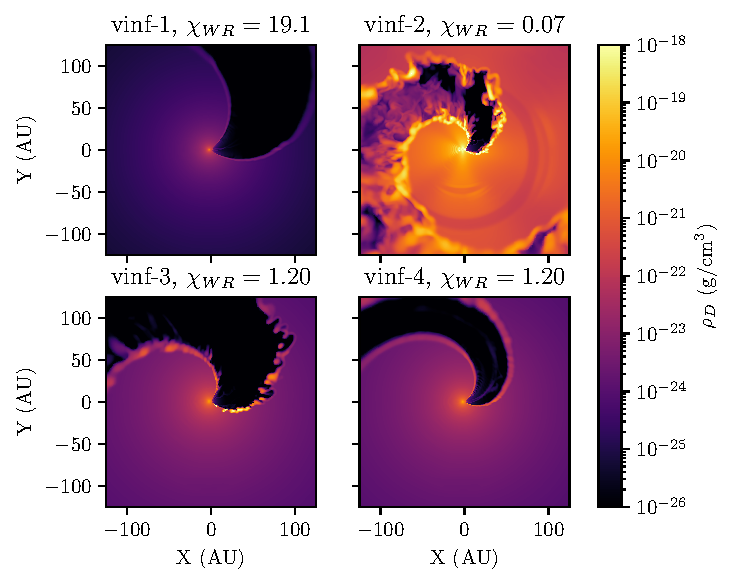
\includegraphics[width=\linewidth]{assets/vinf-finished-rhod.pdf}
      \end{figure}

      \begin{figure}[H]
        \centering
        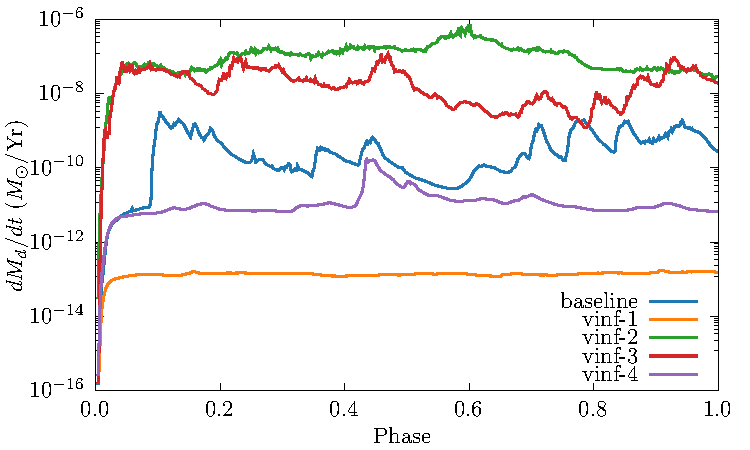
\includegraphics[width=\linewidth]{assets/vinf-phase-dust_rate.pdf}
      \end{figure}

      \section*{Episodic WCd Systems}

      \begin{figure}[H]
        \centering
        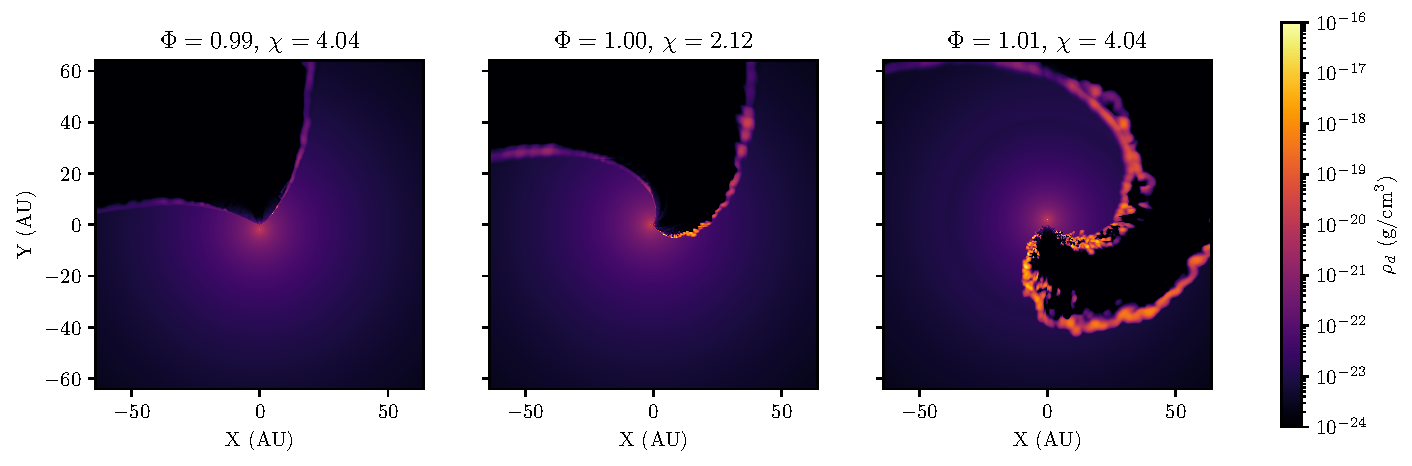
\includegraphics[width=\linewidth]{assets/periastron-3-rhod.pdf}
      \end{figure}

      \begin{figure}[H]
        \centering
        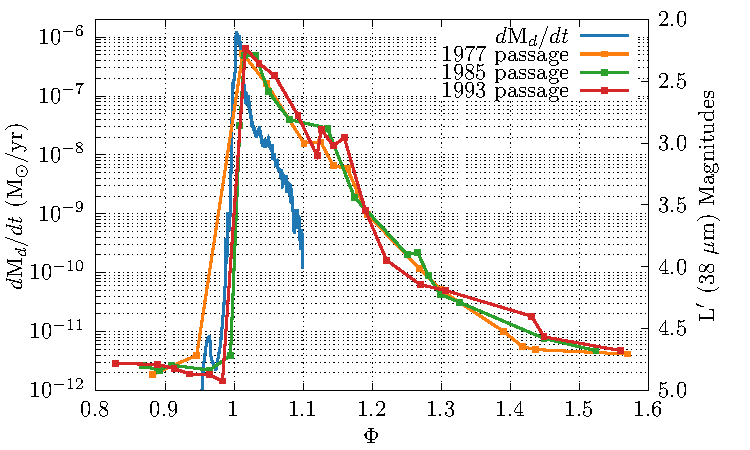
\includegraphics[width=\linewidth]{assets/magnitudes.pdf}
      \end{figure}

      \section*{Future Research}

    \end{multicols}
\end{document}